\chapter{Studio del funzionamento}
\label{cha:analysis}

\section{Il sistema dal punto di vista dell'utente}
\label{sec:ux}

Il sistema FAAC SLH a 2 canali presenta due componenti:
\begin{itemize}
  \item Il ricevitore: una PCB con due pulsanti per gestire tutte le funzioni di memorizzazione dei radiocomandi e 4 dipswitch per gestire la modalità di operazione.
  \item I radiocomandi: semplici trasmettitori a due pulsanti e un led memorizzabili nel ricevitore.
\end{itemize}
Il ricevitore offre una semplice procedura per memorizzare e sincornizzare i radiocomandi, procedura dopo la quale il radiocomando potrà essere utilizzato per il suo scopo. Il sistema FAAC SLH è progettato per essere tollerante: nel caso in cui alcuni segnali del trasmettitore non raggiungano la destinazione, il ricevitore si risincronizzerà (entro alcuni limiti) automaticamente.\\
Inoltre i trasmettitori offrono due funzionalità:
\begin{itemize}
  \item TX coding: un trasmettitore può trasmettere la sua chiave di sistema ad un altro trasmettitore che cambierà la propria chiave di distema in quella appena ricevuta effettivamente clonando il primo.
  \item Master/Slave: di fabbrica un trasmettitore è “master”, ciò vuol dire che può trasmettere la sua chiave di sistema. Tramite la pressione dei pulsanti in una determinata sequenza un master può essere trasformato in “slave”, quest’ultimo viene permanentemente privato della capacità di trasmettere la sua chiave di sistema ma non di assumerne altre.
\end{itemize}
Varie revisioni dei manuali  \cite{man1,man2} dei radiocomandi riportano più o meno informazioni sulle funzionalità dei prodotti.

\section{La trasmissione}
\label{sec:transmission}

\subsection{Segnale ed interpretazione}
\label{sub:signal}

Primo passo nello studio del sistema FAAC SLH è intercettare un segnale per capirne la struttura e la funzione. A questo scopo il Flipper Zero si rivela estremamente utile vista la funzionalità di ricezione di segnali SubGHz già implementata in dettaglio. Utilizzando la funzione “Read RAW” del Flipper Zero possiamo ottenere una lettura non processata del segnale. Questa lettura viene esportata dal Flipper Zero in un file (estensione sub) che riporta le seguenti informazioni:
\begin{itemize}
  \item Filetype: il tipo e contenuto del file
  \item Version: un informazione interna riguardo la versione del’implementazione
  \item Frequenza: la frequenza di ricezione del segnale
  \item Preset: impostazioni di ricezione come modulazione e ampiezza d’onda
  \item Protocollo: il protocollo se risconosciuto (RAW se in modalità raw)
  \item Data: la trasmissione effettivamente ricevuta
\end{itemize}
Per la lettura di un segnale FAAC SLH si usano queste impostazioni:
\begin{itemize}
  \item Frequenza: 433.92MHz
  \item Modulazione: AM270 (rappresenta una modulazione On/Off Keying con ampiezza d’onda di 270kHz)
\end{itemize}
Una lettura così effettuata genererà un file il cui campo “Data” è popolato con una serie di numeri alternativamente positivi e negativi che rappresentano rispettivamente segnale alto e silenzio di lunghezza specificata dal valore assoluto del numero (valore 1 = 1 microsecondo). Osservando queste informazioni si possono estrarre numerose informazioni:
\begin{itemize}
  \item Il segnale del trasmettitore sembra iniziare con un segnale di circa 150ms seguito da un silenzio lungo altrettanto
  \item Una coppia di segnale di 0.3ms e silenzio di 0.3ms viene inviata 8 volte, questa sequenza sembra essere un segnale introduttivo che annuncia l’arrivo della sequenza di dati
  \item una coppia di un segnale lungo 1.1ms e un silenzio lungo altrettanto è inviata, questa sequenza sembra essere un preambolo alla sequenza di dati che rappresenta il payload principale
  \item 64 coppie di segnale e silenzio sono inviate, questa sequenza sembra essere il payload della trasmissione. Queste coppie si configurano in solo due possibili modi:
    \begin{itemize}
      \item Segnale lungo (0.6ms) seguito da silenzio corto (0.3ms)
      \item Segnale corto (0.3ms) seguito da silenzio lungo (0.6ms)
    \end{itemize}
  \item A questo punto il segnale si ripete a partire dal preambolo fino al rilascio del pulsante del trasmettitore
\end{itemize}
Appare quindi chiaro che le 64 coppie segnale-silenzio rappresentino un payload di 64bit in cui ogni coppia rappresenta un bit 1 o 0.\\
Il codice sorgente del firmware del Flipper Zero (sia originale che Unleashed) rivela che:
\begin{itemize}
  \item Segnale corto seguito da silenzio lungo corrisponde al bit 0
  \item Segnale lungo seguito da silenzio corto corrisponde al bit 1
\end{itemize}
A questo punto è triviale ottenere il payload a partire da questi dati, una funzione per ciò è già implementata nel Flipper Zero nel file \texttt{lib/subghz/protocols/faac\_slh.c}\cite{firmware}.

\subsection{Struttura del pacchetto dati}
\label{sub:payload}
D’ora in poi con il termine “chiave” si intenderà il pacchetto dati di 64 bit inviato dal trasmettitore.\\
Il trasmettitore FAAC SLH può trasmettere due chiavi differenti:
\begin{itemize}
  \item Chiave normale: inviata alla pressione normale di uno dei pulsanti, è il pacchetto standard inviato quando il radiocomando deve autenticarsi nel ricevitore.
  \item Chiave di programmazione: inviato alla pressione di uno dei pulsanti mentre il trasmettitore è in modalità “Programmazione”, all’interno del codice del firmware “Unleashed” viene soprannominato “Master Remote Prog Key”.
\end{itemize}
Analizziamo prima la chiave normale che, secondo la rappresentazione esadecimale di 64 bit, prenderà questa forma:
\begin{center}
  \texttt{XX XX XX XY ZZ ZZ ZZ ZZ}
\end{center}
I 4 byte più significativi (\texttt{XX XX XX XY}) rappresentano quello che viene soprannominato “code fix”. Questa porzione contiene il numero seriale, detto “serial”, del trasmettitore (\texttt{XX XX XX X}, 28 bit) e il valore del tasto premuto (\texttt{Y}, 4 bit), detto “button”. Chiaramente il serial non varia mai per un trasmettitore mentre il button varia in base al pulsante premuto\footnote{Il code fix può cambiare quando il radiocomando è trasformato in slave ma mai in operazione normale}.\\
4 byte (32 bit) meno significativi (\texttt{ZZ ZZ ZZ ZZ}) rappresentano quello che viene soprannominato “code hop”, ovvero il codice a rotazione in sé. Ovviamente il code hop cambia ad ogni trasmissione.\\
Si potrebbe pensare a questi due elementi come l’username (il code fix) e la password (il code hop) di un tradizionale login form.
Si è rilevato che il ricevitore apparentemente accetti esclusivamente trasmettitori con valore serial entro il range [A0000000--A0FFFFFF] in questa maniera:\\
\begin{itemize}
  \item Si emulano vari radiocomandi FAAC SLH tramite la funzionalità “Add manually” > “Faac SLH 433MHz” sul Flipper Zero (firmware Unleashed necessario)
  \item Si inviano vari segnali con vari differenti valori di “code fix”, count invariato e seed invariato
  \item Si osserva che solo valori di code fix compresi nel range precedentemente menzionati si autenticano correttamente nel ricevitore.
\end{itemize}
Non può essere escluso che altri valori vengano accettati dal ricevitore vista l’implausibilità di testare tutte le combinazioni di 32 bit, tuttavia è ragionevole pensare che sia l’implementazione effettiva interna al ricevitore. Il range sopra menzionato offre 16\^6 possibili code fix.\\
Analizziamo ora la chiave di programmazione che prende questa forma:
\begin{center}
  \texttt{52 0F XX XX XX XX YY 00}
\end{center}
Si può osservare come questa chiave sia contraddistinta dai primi 2 byte più significativi e dal byte meno significativo che rimangono costanti a qualsiasi trasmissione di questo tipo. Si può ipotizzare che sia questo il meccanismo con cui il ricevitore riconosce il tipo di chiave ricevuta.\\
Il contenuto di questa chiave è diviso in \texttt{XX XX XX XX} che rappresenta il valore del seed codificato e \texttt{YY}, valore che viene chiamato mCnt necessario alla decodifica del seed.\\
La chiave è trasferita in modalità Big Endian.

\section{Implementazione del codice a rotazione}
\label{sec:rolling}

\subsection{KeeLoq}
\label{sub:keeloq}

Fonti: \cite{keeloqwiki,keeloqc,algebraic_slide,cryptoeprint,periodic_ciphers}.\\

\begin{wrapfigure}
  {r}{.5\textwidth} %
  \centering
  \def\stackalignment{r}\stackunder{
    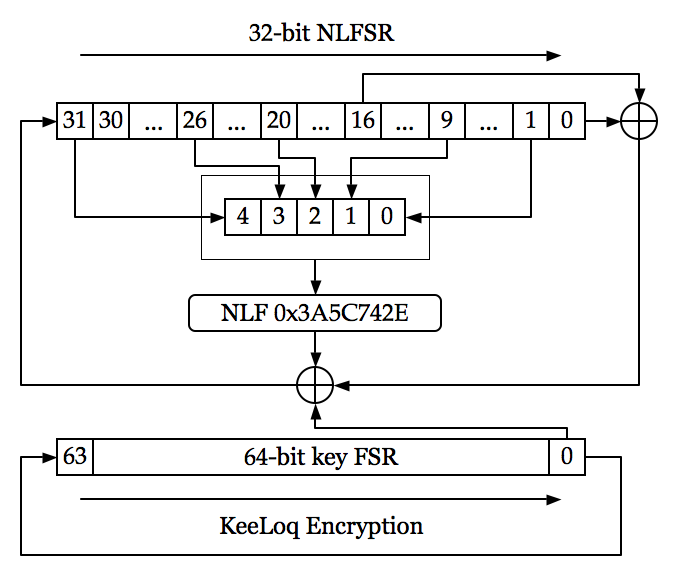
\includegraphics[width=\linewidth]{images/encrypt.png}
  } %
  {\scriptsize \parbox[t]{\linewidth}{ Fonte: \cite{keeloqwiki}} }
  \caption{Fase di encrypt in KeeLoq}
  \label{fig:keeloq_encrypt}
\end{wrapfigure}
Come menzionato precedentemente FAAC SLH sfrutta l’algoritmo KeeLoq per l’implementazione del codice a rotazione. Ai fini di questo studio non è necessaria una conoscenza troppo approfondita di questo algoritmo, difatti si potrebbe semplicemente considerarlo un black box algorithm che prende in input un payload e la chiave ed è in grado di crittografare o decrittografare i dati. Tuttavia risulta utile comprenderne a grandi linee il funzionamento per capire come FAAC SLH lo integra.\\
Keeloq, a partire dagli anni ‘80, gode di ampio utilizzo in sistemi di RKE per veicoli, barriere fisiche e sistemi di allarme.\\
L’algoritmo KeeLoq sfrutta due registri da 32 bit (stato) e 64 bit (chiave) che, rispettivamente, operano come Non-Linear Feedback Shift Register (NLFSR) e registro circolare e, sempre rispettivamente, sono inizializzati con il plaintext e la chiave segreta. Un initialization vector (IV) è utilizzato in certe implementazioni per inizializzare il registro a 32 bit e garantire un cifrario differente per lo stesso messaggio.
Il ciclo principale di crittografia dell’algoritmo è composto di 528 iterazioni per ognuna delle quali il feedback dell’NLFSR dipende da i bit 1, 9, 20, 26 e 31 del registro di stato e da una specifica Non-Linear Feedback Function (NLF) data da: \(NLF(a, b, c, d, e) = d \oplus e \oplus ac \oplus ae \oplus bc \oplus be \oplus cd \oplus de \oplus ade \oplus ace \oplus abd \oplus abc\), funzione rappresentabile dall’esadecimale 0x3A5C742E. L’output di questa funzione viene quindi combinato linearmente (XORed) con i bit 0 e 16 del NLFSR e dal bit 0 del registro chiave nel suo attuale stato. Il risultato di questa serie di operazioni viene reinserito nel NLFSR. Dopo ogni iterazione entrambi i registri scorrono di un bit a destra. Il risultato finale si ottiene dallo stato finale del registro di stato dopo le 528 iterazioni. Il vettore di inizializzazione del registro di stato è tipicamente sottoposto a XOR con i bit meno significativi della chiave sia prima che dopo le iterazioni.\\

\begin{wrapfigure}
  {r}{.5\textwidth} %
  \centering
  \def\stackalignment{r}\stackunder{
    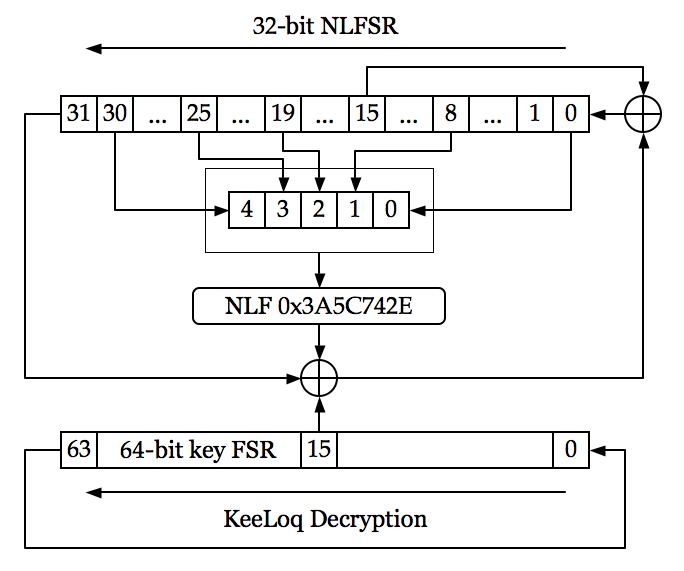
\includegraphics[width=\linewidth]{images/decrypt.png}
  } %
  {\scriptsize \parbox[t]{\linewidth}{ Fonte: \cite{keeloqwiki}} }
  \caption{Fase di decrypt in KeeLoq}
  \label{fig:keeloq_decrypt}
\end{wrapfigure}

Il processo di decrittografia avviene in maniera simile a quello di crittografia con alcune differenze chiave:
\begin{itemize}
  \item Il registro di stato è inizializzato con il testo cifrato
  \item La NLF dipende da un insieme diverso di bit di stato: 0, 8, 19, 25 e 30
  \item L’output della NLF è sottoposto a XOR con bit differenti dello stato (31 e 15) e della chiave (15)
  \item Il registro di stato scorre verso sinistra
\end{itemize}
Seppure la NLF introduca un fattore di non linearità è facile notare la semplicità della struttura e la lunghezza relativamente limitata della chiave a 64 bit. Inoltre vari attacchi criptoanalitici hanno sfruttato l’esistenza di approssimazioni lineari efficienti della NLF ed il fatto che l’utilizzo e l’aggiornamento della chiave dopo 64 round si ripete.

\subsection{KeeLoq in FAAC SLH}
\label{sub:faacslh}

Per comprendere l’implementazione di KeeLoq a rotazione di FAAC SLH osserviamo il procedimento di memorizzazione nel ricevitore, il contenuto della chiave di programmazione e il codice sorgente del firmware Unleashed.\\
Il procedimento per memorizzare il trasmettitore nel ricevitore si compone di queste fasi:
\begin{itemize}
  \item Tramite un pulsante sul ricevitore si imposta quest’ultimo in modalità “Programmazione”
  \item Si invia una chiave di programmazione con il trasmettitore, il ricevitore quindi uscirà dalla modalità programmazione
  \item Si inviano due chiavi normali col trasmettitore e alla seconda ricevuta il ricevitore sarà sincronizzato e aprirà la barriera
\end{itemize}
Ricordiamo il formato della chiave di programmazione:
\begin{center}
  \texttt{52 0F XX XX XX XX YY 00}
\end{center}
in cui \texttt{XX XX XX XX} è il seed codificato e \texttt{YY} è una chiave di decodifica.
La routine della decodifica del seed si compone di un ciclo che itera sul valore del seed codificato YY volte il cui corpo è composto di semplici manipolazioni bitwise del valore in funzione di mCnt. Questo routine sembra un modo di offuscare il valore del seed durante la trasmissione ma risulta, tuttavia, estremamente debole.\\
Il codice responsabile di questo processo nel firmware Unleashed è riportato nell'appendice A.\\
Una volta ottenuto il seed, il ricevitore esce dalla modalità di programmazione e torna in modalità di ascolto normale, si può quindi supporre che il seed venga salvato internamente per inizializzare un counter interno.\\
Le successive due chiavi normali trasmesse, se sequenziali, sincronizzeranno il ricevitore con il trasmettitore.\\
Ricordiamo ora la struttura delle chiavi normali:
\begin{center}
  \texttt{XX XX XX XX YY YY YY YY}
\end{center}
dove \texttt{XX XX XX XX} è detto “code fix” e \texttt{YY YY YY YY} è detto “code hop”.\\
Il code fix è composto a sua volta da numero seriale “serial” e pulsante premuto “btn” ma a livello di funzionalità del ricevitore non è necessario distinguere queste due parti.\\
Il codice del firmware Unleashed offre l’implementazione di KeeLoq in FAAC SLH per la decrittografia del code hop. Ricordiamo che l’algoritmo di KeeLoq crittografa un payload di 32 bit con una chiave di 64 bit. La chiave di 64 bit è ottenuta nella seguente funzione a partire dal seed e dalla cosiddetta “Manufacturer key”, una chiave costante segreta legata a FAAC SLH.\\
É interessante il fatto che per ottenere la chiave da 64 bit la funzione di learning esegua l’intero algoritmo di KeeLoq nella versione di encrypt due volte.\\
Ottenuta la chiave di 64 bit si estrae il valore del counter dal risultato della decrittografia.\\
Il codice di questi vari procedimenti è riportato nell'appendice B.\\
Due note:
\begin{itemize}
  \item Il count è composto di solo 5 cifre esadecimali (5 nibble)
  \item A volte la lettura della chiave di programmazione di un singolo radiocomando effettuata col Flipper Zero riporta un risultato peculiare differente dal normale: se il seed di un radiocomando è \texttt{XX XX YY YY} a volte \texttt{YY YY XX XX} viene letto. Non è chiaro se questo fatto risulti da un errore nell’implementazione del protocollo nel firmware Unleashed o se sia un comportamento anomalo del radiocomando.
\end{itemize}
In base a quanto dedotto dal codice del firmware, il code fix non entra in gioco nel processo di decodifica del valore count, infatti, come sarà spiegato successivamente, il ruolo di questo valore è cruciale nella sincornizzazione di multipli radiocomandi sullo stesso ricevitore.\\
É importante sottolineare come il processo appena descritto avviene nel Flipper Zero durante la lettura dei segnali FAAC SLH e non nel ricevitore originale FAAC SLH: è altamente probabile che internamente il ricevitore segua una logica ben differente quando si tratta di decriptare ed autenticare i segnali ricevuti, tuttavia la logica di KeeLoq rimane valida. Per esempio si potrebbe ipotizzare che il ricevitore decripti il segnale ricevuto dal radiocomando e verifichi il valore del counter, oppure che il ricevitore stesso calcoli il code hop previsto e verifichi che quello ricevuto corrisponda.\\

\subsection{L'autenticazione}
\label{sub:auth}

\begin{wrapfigure}
  {r}{.5\textwidth} %
  \centering
  \def\stackalignment{r}\stackunder{
    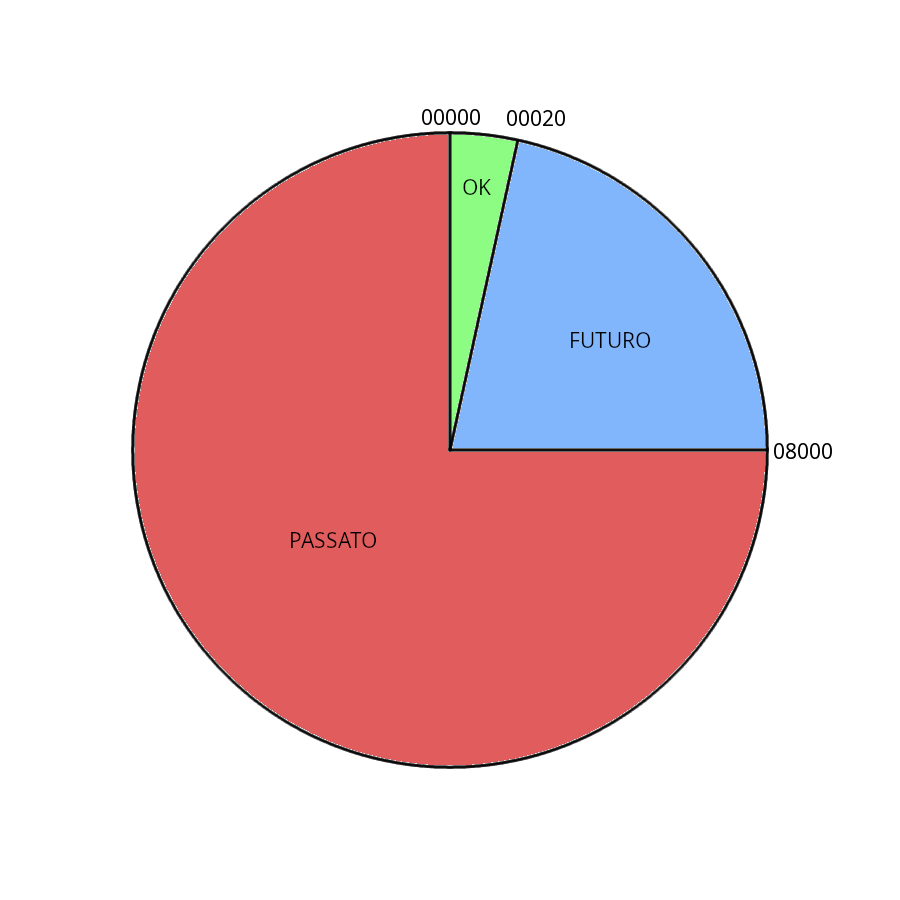
\includegraphics[width=\linewidth]{images/count_pie.png}
  } %
  {\scriptsize \parbox[t]{\linewidth}{Intervalli non in scala}}
  \caption{Il counter circolare}
\end{wrapfigure}

Come menzionato precedentemente, FAAC SLH è progettato per essere tollerante a desincronizzazioni entro un certo limite.\\
Ricordando che non possiamo conoscere effettivamente il funzionamento interno del ricevitore, ipotizziamo che alla ricezione di un segnale lo decripti tramite l’algoritmo precedentemente descritto e confronti il valore del counter ricevuto con un valore interno mantenuto in una qualche memoria, alcune proprietà possono essere osservate effettuando specifiche emulazioni di radiocomandi con il Flipper Zero.
Prima di tutto si può osservare che il counter interno del ricevitore deve essere composto di soli 20 bit (5 cifre esadecimali) seppure durante l’emulazione del radiocomando il Flipper permetta di inserire valori nel counter di 6 cifre esadecimali. Questo si può dedurre dal fatto che radiocomandi con valori di count \textsl{0x0yyyyy}, \texttt{0x1yyyyy}, etc autenticano tutti correttamente sul ricevitore.\\
In secundis, il valore di count ha un comportamento ciclico: arrivato al valore \texttt{0xFFFFF} il counter ritorna al valore \texttt{0x00000} e continua ad autenticare correttamente.\\
Il ricevitore accetta valori del count che distano di massimo 0x20 (32) valori dopo l’ultimo autenticato.\\
Oltre i 32 valori accettati ed entro 0x8000 (32768) valori dopo l’ultimo autenticato il segnale è considerato futuro. In questo caso il ricevitore non autentica il radiocomando ma tenta una resincronizzazione. Per resincronizzare il counter interno del ricevitore è necessaria un’altra chiave normale futura entro il range precedentemente menzionato di futuro e appena successiva, cioè il counter della seconda chiave deve essere esattamente successivo a quello della prima futura. La necessità di due chiavi sequenziali per la resincronizzazione al futuro restringe il massimo valore che può avere un radiocomando per resincronizzare il ricevitore a counter + 0x7FFF.\\
Un comportamento interessante si può osservare inviando una sequenza di 4 chiavi di questo tipo: chiave accettabile > chiave futura > chiave accettabile > chiave futura. Elenchiamo i comportamenti del ricevitore ad ogni chiave ricevuta:
\begin{itemize}
  \item Alla prima accettabile il ricevitore autentica correttamente
  \item Alla prima chiave futura il ricevitore non autentica il radiocomando
  \item Alla seconda chiave accettabile il ricevitore autentica il radiocomando: questo implica che il contatore interno del ricevitore non è aggiornato al futuro alla prima chiave futura ricevuta, tuttavia potrebbe essere in uno stato in cui attende anche una possibile chiave futura in sequenza alla precedente
  \item Alla seconda chiave futura il ricevitore autentica il radiocomando futuro e si risincronizza a tale futuro, il radiocomando precedentemente accettabile non viene più autenticato
\end{itemize}
Questi comportamenti sembrano puntare alla possibilità che il ricevitore tenga in memoria una cronologia di chiavi passate ricevute. Per testare la lunghezza di questa cronologia vengono inviati al ricevitore una chiave futura che non autentica, un numero variabile crescente di chiavi accettabili e, infine, una chiave esattamente successiva alla prima. Cominciando con una sola chiave accettabile tra le due future si aumenta il numero di chiavi accettabili fino a quando la seconda chiave futura (l’ultima della sequenza) smette di risincronizzare il ricevitore. Purtroppo, dopo numerosi tentativi questo metodo non ha portato risultati conclusivi: ripetendo più volte lo stesso esperimento il ricevitore ha smesso di risincronizzare dopo differenti numeri di chiavi accettabili centrali, tuttavia sembra non superare mai il numero di 8 chiavi passate mantenute nella cronologia. É importante sottolineare come ad ogni test di questo tipo effettuato la memoria del ricevitore è svuotata secondo la procedura esplicata nel manuale e successivamente reinizializzata ad un radiocomando emulato, c’è la possibilità che ogni inizializzazione di memoria definisca una lunghezza della memoria differente o, più probabilmente, ognuna delle ripetizioni del segnale trasmesse dal radiocomando sia registrata nella cronologia. In ogni caso non si può essere certi della lunghezza effettiva della cronologia.\\
Il procedimento di risincronizzazione in caso di chiave futura sembra essere molto simile al processo di memorizzazione del radiocomando. Questo processo verrà dettagliato nel capitolo successivo, dove si avranno più informazioni per fare ipotesi più informate.\\

\section{Funzionalità: TX coding e master/slave}
\label{sec:func}

Il radiocomandi FAAC SLH mettono a disposizione due meccanismi utili alla comodità di utilizzo e ad aumentare la versatilità del sistema.\\
Analizziamo per prima la funzionalità di TX coding che, in base al comportamento osservato, sembra essere funzionale alla meccanica master/slave. Come discusso precedentemente, un radiocomando in modalità programmazione invia un payload contenente il proprio seed. Secondo una procedura descritta nel manuale di utilizzo dei radiocomandi [INSERIRLO], un radiocomando può assumere il seed di un altro radiocomando così da poter autenticarsi correttamente nei ricevitori che già avevano memorizzato l’altro radiocomando. In base a letture effettuate tramite il Flipper Zero delle trasmissioni del radiocomando a cui è stato cambiato il seed seguendo il procedimento di TX coding si conferma il comportamento atteso: il seed del radiocomando ricevente viene sostituito dal seed del radiocomando programmante.\\
Analizziamo ora la funzionalità master/slave, seppur poco rilevante allo scopo di questo studio. Un radiocomando FAAC SLH esce di fabbrica in modalità “master”, da manuale \cite{man1} e come osservabile in base al comportamento, si deduce che questa modalità implica la capacità del radiocomando di trasmettere la chiave di programmazione. Il radiocomando può essere trasformato in uno “slave” seguendo un semplice procedimento descritto nel manuale, in questa modalità perderà la capacità di trasmettere il seed, pur continuando ad operare nella stessa maniera per quanto riguardo il resto delle funzionalità. Il radiocomando sembra anche cambiare il proprio valore serial quando trasformato in uno slave, mantenendosi comunque nel range [A0000000--A0FFFFFF].\\
Chiaramente queste funzionalità sono sviluppate al fine di semplificare l’utilizzo del sistema alla necessità di multipli radiocomandi per un singolo ricevitore: come spiegato nel manuale, una volta che il corretto seed è registrato in un radiocomando (tramite la meccanica di TX coding appena descritta) è sufficiente inviare due chiavi in sequenza perché il ricevitore cominci ad autenticare un nuovo radiocomando insieme a tutti gli altri già precedentemente registrati. Il ricevitore, chiaramente, non accetta due radiocomandi con lo stesso code fix ma count differenti perché, in questo caso, si incapperebbe nel controllo del valore del count che non necessariamente coincide tra i due.\\
Il funzionamento di questa meccanica fornisce un'importante intuizione sul funzionamento interno del ricevitore: a patto che il ricevitore non abbia memorizzato il massimo numero di radiocomandi, al fine di aprire la barriera controllata dal ricevitore è necessario un qualsiasi segnale che fornisca un code hop valido e abbia un code fix differente da altri già memorizzati, più semplicemente il segnale deve essere generato a partire dal seed memorizzato nel ricevitore e avere un code fix non già memorizzato, il ricevitore si occuperà in questo caso di sincronizzare un nuovo radiocomando in base ai segnali ricevuti.\\

\section{Ipotesi informata sul funzionamento interno del ricevitore}
\label{sec:ipothesis}

In base alle osservazioni fino ad ora descritte si può assumere un processo di autenticazione dei radiocomandi interno al ricevitore che segue questi passi in ordine:
\begin{itemize}
  \item Alla ricezione di un segnale il ricevitore controlla il valore del counter della chiave ricevuta (o decifrando il segnale o controllando se uno dei possibili code hop validi ottenibili da seed e counter entro un certo range corrisponde con quello ricevuto).
  \item Nel caso in cui il counter ricevuto rientri nel range di valori validi per uno dei code fix salvati in memoria il ricevitore controlla se il code fix della chiave ricevuta corrisponde a quella del ricevitore corrispondente al code fix appena menzionato, in caso positivo la barriera viene aperta e il counter di tale entry in memoria aggiornato.
  \item Altrimenti, nel caso in cui il counter ricevuto rientri nel range di valori futuri per una delle entries in memoria lo stesso controllo del caso precedente viene eseguito ma il ricevitore attiva la modalità resync.
  \item In una qualsiasi altra situazione il ricevitore non reagisce.
\end{itemize}
Ad una ricezione con la modalità resync attivata si può ipotizzare che il ricevitore controlli la presenza, nella cronologia delle ricezioni descritta precedentemente, di una chiave immediatamente precedente a quella appena ricevuta (con code fix corrispondente).\\
Si può inoltre ipotizzare che l’inizializzazione del sistema avvenga in questa maniera:
\begin{itemize}
  \item Il ricevitore riceve una chiave di programmazione e memorizza il seed decifrato nella propria memoria
  \item Il ricevitore attiva una modalità di programmazione di un nuovo radiocomando
\end{itemize}
Infine, si può ipotizzare che la memorizzazione di un nuovo radiocomando, sia in caso di prima memorizzazione che altrimenti, sia simile alla procedura di resync, ma invocata senza un limite al range del valore del counter.

\section{Un possibile attacco brute-force contro FAAC SLH}
\label{sec:attack}

Le funzionalità descritte precedentemente aprono la possibilità di un bruteforce attack viste alcune caratteristiche del sistema FAAC SLH.\\
Ricordiamo tali caratteristiche del sistema:
\begin{itemize}
  \item Il ricevitore si sincronizza con qualsiasi radiocomando contenente il seed corretto tranne al più radiocomandi con un code fix già memorizzato
  \item Nel processo di autenticazione il code fix è rilevante solo dopo aver eventualmente trovato un valore di count accettabile o futuro
\end{itemize}
Di conseguenza, catturando due segnali consecutivi da un radiocomando genuino, un algoritmo (come suggerito in una chat privata dal creatore del firmware Unleashed) potrebbe iterare l’algoritmo KeeLoq (versione FAAC SLH) per ogni possibile valore del seed (2\^32) per ogni possibile valore del counter (2\^20) finché non trova una sequenza di due valori di code hop indentica a quella catturata. A questo punto, ottenuto il seed, si può sfruttare il funzionamento del ricevitore per sincronizzare un memoria un nuovo radiocomando in idealmente pochi tentativi o addirittura clonare il radiocomando catturato e riniscronizzarlo ad un futuro prossimo.\\
Va sottolineato il fatto che questa possibilità si presenta solo dal momento che la Manufacture key di FAAC SLH è nota, altrimenti un ulteriore spazio di 2\^32 valori dovrebbe essere testato.\\
Questo approccio deve coprire uno spazio di 2\^32 * 2\^20 valori (tutti seed e count possibili), risulta quindi non realisticamente fattibile in tempi brevi su CPU, più plausibile è un’implementazione che sfrutta accelerazioni hardware come OpenCL, ROCm, HIP p CUDA.\\
Assumendo una GPU Nvidia RTX 3080 con una frequenza di clock di 2 Ghz e 8704 core e assumendo un implementazione assembly ottimizzata che impiega 2200 (nota a piè di pagina n. 4 in \cite{cryptoeprint}) cicli di clock per una intera crittografia KeeLoq si può coprire l’intero spazio delle chiavi in un tempo massimo di 160 ore, non pratico ma non implausibile. Tale algoritmo di bruteforce ignora inoltre numerose possibilità come approssimazioni lineari della Non Linear Function di KeeLoq e techniche di scorrimento ed algebriche che potrebbero ridurre notevolmente il tempo di esecuzione \cite{cryptoeprint,algebraic_slide,attack,periodic_ciphers}.
Un programma in CUDA proof-of-concept di questa idea è riportato in appendice C con la manufacturer key di FAAC oscurata per questioni legali.
